\documentclass[conference]{IEEEtran}
\usepackage[utf8]{inputenc}
\usepackage{graphicx}
\usepackage{booktabs}
% No hyperref: the call forbids embedded links, so URLs stay plain text.
\usepackage{url}
\title{AirGuard India: A Provenance-Aware Prospective Air-Quality Forecasting System}
\author{\IEEEauthorblockN{Nishanth R, NAME, NAME}
\IEEEauthorblockA{Affiliations and author consent pending human confirmation}}
\begin{document}
\maketitle
\begin{abstract}
This is an unsubmitted research draft describing a working live data system and
a prospective evaluation protocol. The system separates observed station data,
modelled concentrations, weather context and satellite fire detections. It
retains issue-time provenance and excludes retrospective substitutions from
forecast validation. Historical archive access and sufficient matched station
outcomes are pending; consequently this draft makes no claim of improved
forecast accuracy, calibrated uncertainty or clinical benefit.
\end{abstract}
\begin{IEEEkeywords}air quality, provenance, prospective forecasting, India\end{IEEEkeywords}
\section{Problem and Scope}
A historical replay cannot establish today's conditions. A retrieved model
forecast is also distinct from a measured station observation. AirGuard's
operational interface keeps source identity, freshness and aggregation method
visible. This draft describes implementation and preregistration, not completed
national validation.
\section{Related Work}
Health-weighted indices are not new. The Canadian AQHI combines pollutants
through short-term mortality associations rather than a maximum sub-index
\cite{stieb2008aqhi}, and a city-specific AQHI has been constructed for Delhi and
Varanasi from Indian mortality series \cite{george2025aqhi}. Indian short-term
mortality coefficients are available at multi-city scale \cite{debont2024india},
alongside systematic-review estimates \cite{orellano2020shortterm}. This work
therefore claims no first health-weighted index. The intended contribution is the
combination of a forecast, station calibration, calibrated uncertainty and cohort
advisories under an issue-time protocol, and that combination is not yet
evidenced.

Operational forecasting in India exists at city scale, including a
high-resolution Delhi system \cite{jena2021delhi}, and regional models are
reported to overestimate surface ozone over India \cite{pommier2018india}. Recent
work forecasts particulate matter over the subcontinent from CAMS fields without
ground stations \cite{kushwaha2025nowcasting}. The global forecast used here is
the CAMS composition product \cite{cams2024forecasts}, which is distinct from the
CAMS reanalysis \cite{inness2019camsra}: the reanalysis may be used
retrospectively but never as a forecast input. Measured observations arrive
through OpenAQ \cite{openaq2026} and forecast fields through Open-Meteo
\cite{openmeteo2026}; neither is a CPCB export.

Planned uncertainty quantification follows adaptive conformal inference
\cite{gibbs2021aci}, with an ensemble batch alternative for time series
\cite{xu2021enbpi}. Model comparison will use Diebold--Mariano tests
\cite{diebold1995comparing} and proper scoring rules \cite{gneiting2007scoring};
feature attribution, where reported, is descriptive \cite{lundberg2017shap}.
Retrospective event analysis will use random-forest meteorological normalisation
\cite{grange2018normalisation}, as applied to lockdown air quality
\cite{shi2021lockdown}. The index definition follows the CPCB national method
\cite{cpcb2014aqi}, and guideline values are those of the World Health
Organization \cite{who2021guidelines}.

\section{Data and Provenance}
OpenAQ measurements preserve upstream station identity and licence metadata.
Open-Meteo supplies CAMS global pollutant concentrations and weather forecasts.
NASA FIRMS supplies fire context only. CPCB ingestion is unavailable on the
current network. Archived issue-time CAMS inputs are pending ADS access; current
forecast fields or reanalysis must not replace that archive.
\section{Method and Issue-Time Controls}
A central CPCB-style calculation uses adequately covered pollutant windows and
reports open-ended severe bands as lower bounds. Hourly relative exposure
windows use instantaneous concentration-derived indicators within practical
hours; they are not official hourly AQI or a safety threshold. The fixed-time
prospective protocol freezes inputs available by 20:00 IST for the next IST
calendar day, binds a station before the outcome and rejects backdating.
\section{Preregistered Evaluation}
The expanded study requires at least 100 eligible stations, 365 training days,
30 calibration days, rolling temporal folds with an embargo and a locked latest
90-day final test. Spatial, region and coastal holdouts, pollutant correction,
uncertainty calibration and advisory trade-offs require actual matched records.
Persistence, climatology and raw CAMS remain baselines. Candidate improvements
must be assessed against these baselines using date-blocked comparisons.
\section{Available Evidence and Limitations}
% Generated by scripts/export_evidence_table.py. Do not edit by hand.
% Generated 2026-10-11T16:28:50.227084+00:00 from the artefacts named in each row.
\begin{table}[t]
\caption{Evidence actually held. Record counts do not establish predictive skill, and a
station-year of a single pollutant cannot produce a CPCB daily AQI.}
\label{tab:evidence}
\centering
\begin{tabular}{lr}
\toprule
Evidence & Count \\
\midrule
Measured hourly records audited & 267 \\
Eligible issue-time forecast/target pairs & 0 \\
Stations with 365 candidate complete days & 0 \\
Archive hourly records collected & 72,339 \\
Station-days with a valid CPCB-style daily AQI & 861 \\
Stations with one year of valid daily targets & 0 \\
Fixed-time prospective forecasts issued & 12 \\
Verified prospective outcomes & 0 \\
\bottomrule
\end{tabular}
\end{table}

\begin{figure}[t]
\centering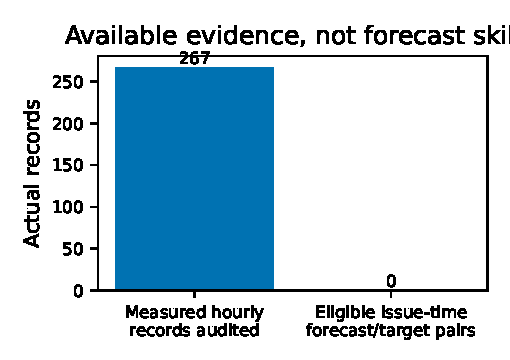
\includegraphics[width=\columnwidth]{figures/evidence_coverage.pdf}
\caption{Available records in the audit snapshot. Record counts do not establish
predictive skill.}\end{figure}
No empirical national accuracy, interval coverage, health benefit, population
impact or deweathered causal estimate is currently supported. The operational
forecast remains a clearly labelled CAMS-based estimate. Source resolution,
missing station coverage, correlated samples and availability timestamps limit
interpretation. Prospective evidence must accumulate before deployment of an
India-specific correction.
\section{Cohort Advisory Index}
The legacy advisory index multiplied CPCB sub-indices by cohort factors chosen by
hand, so its divergence from the official index followed in part from that
choice. The replacement is an excess-risk form, $\mathrm{ER} = \sum_p
(\exp(\beta_p C_p) - 1)$, reported on the official 0--500 scale and anchored so
that a reference adult on a CPCB band boundary reads that boundary. The anchoring
matters: without it, changing the index form produces a difference from the
official index by itself. Every coefficient $\beta_p$ and every cohort modifier
is unadopted pending evidence review, the framework returns no value until one is
adopted, and Table~\ref{tab:hai_factors} is generated from that register rather
than typed.
% Generated by scripts/export_hai_factors.py. Do not edit by hand.
\begin{table}[t]
\caption{HAI v2 coefficient register. No concentration--response coefficient is adopted:
each entry awaits verification of its source, exposure window, population and units.}
\label{tab:hai_factors}
\centering
\begin{tabular}{llll}
\toprule
Pollutant & Window & Coefficient & Source \\
\midrule
PM2.5 & 24h\_mean & Awaiting evidence review & -- \\
PM10 & 24h\_mean & Awaiting evidence review & -- \\
NO2 & 24h\_mean & Awaiting evidence review & -- \\
SO2 & 24h\_mean & Awaiting evidence review & -- \\
CO & max\_8h\_running\_mean & Awaiting evidence review & -- \\
O3 & max\_8h\_running\_mean & Awaiting evidence review & -- \\
NH3 & 24h\_mean & Neutral by declaration & -- \\
Pb & 24h\_mean & Neutral by declaration & -- \\
\midrule
\multicolumn{4}{l}{\footnotesize Cohort effect-modification factors} \\
\midrule
healthy adult & reference & all factors 1.0 (no evidence adopted) & -- \\
children & unverified & all factors 1.0 (no evidence adopted) & -- \\
elderly 60plus & unverified & all factors 1.0 (no evidence adopted) & -- \\
asthma copd & unverified & all factors 1.0 (no evidence adopted) & -- \\
cardiac & unverified & all factors 1.0 (no evidence adopted) & -- \\
pregnant & unverified & all factors 1.0 (no evidence adopted) & -- \\
outdoor worker & unverified & all factors 1.0 (no evidence adopted) & -- \\
\bottomrule
\end{tabular}
\end{table}

A cohort reading that differs from the official index is a property of the index.
It is not evidence of health benefit, and no outcome validation is claimed.

\section{Conclusion and Submission Gate}
The live system and evidence ledger are implemented. Submission requires real
matched evaluation evidence, author consent, an applicable conference call and a
checked six-page PDF. This source is intentionally not presented as a finished
six-page paper. The bibliography is generated from Crossref, the arXiv API and
official publisher pages and each entry was checked against its expected title;
whether a cited source supports the claim attached to it remains the authors'
judgement.

\section*{Ethics Statement}
No human-subject data was collected. The comprehension study described in the
repository's study protocol is not authorised to collect data and will not run
before institutional ethics approval and informed consent. The cohort advisory
index is a heuristic, not medical advice, and it is not validated against any
health outcome.

\section*{Acknowledgment}
Measured observations are provided by OpenAQ and its upstream operators,
forecast fields by Open-Meteo from the Copernicus Atmosphere Monitoring Service,
and fire detections by NASA FIRMS. The index method follows the Central
Pollution Control Board.

\textbf{AI use disclosure.} Anthropic Claude (Claude Code) and OpenAI Codex were
used as coding and drafting assistants: for the software, tests and evidence
scripts described here, and for drafting prose in the Related Work, Method,
Cohort Advisory Index, Limitations and Conclusion sections, which the authors
then revised. Every number in this paper is produced by a committed script from
versioned data; no result was typed by hand. Bibliography entries were retrieved
programmatically and verified against publisher records rather than edited by
hand. The authors are responsible for the entire content of this paper.

\bibliographystyle{IEEEtran}
\bibliography{refs}
\end{document}
